\documentclass[titlepage]{report}
\usepackage[]{multipack}

\title{Title}
\author{Schippers, C.F.}
\date{\today}

\begin{document}
\setAbstract{}
\inserttitletoc

\listoftodos
\newpage

\chapter{Theoretical exercises}
\section{Exercise 1}
\todo{opgaven maken}

\section{Exercise 2}
\subsection{a}
\begin{equation}
	U = 4 \varepsilon \left[ \left(\frac{\sigma}{r}\right)^{12} - \left(\frac{\sigma}{r}\right)^6\right].
\end{equation}

Take the derivative to $ r $ and put to zero for $ r = r\sub{min} $
\begin{equation}
	\left. \pd{U}{r} \right|_{r=r\sub{min}} = 4 \varepsilon \left[ -12 \frac{\sigma^{12}}{r\sub{min}^{13}} + 6\frac{\sigma^{6}}{r\sub{min}^{7}} \right] = 0.
\end{equation}

This solves to
\begin{equation}
	r\sub{min} = \sqrt[6]{2} \sigma.
\end{equation}

Putting this in $ U $ gives
\begin{equation}
	U\left(r = r\sub{min}\right) = - \varepsilon.
\end{equation}

\subsection{b}
$ D_e $ is the depth of the potential well. 
A Taylor-expansion of the potential around $ l = l_0 $ gives
\begin{subequations}
	\begin{align}
		v(l) =& D_e \left[ 1 - \exp\left(-a (l-l_0)\right) \right]^2 \\
		\approx& a^2 D_e (l-l_0)^2 + \mathcal{O}\left((l-l_0)^3\right).
	\end{align}
\end{subequations}
So at small deviations from $ l_0 $ the Morse potential is approximately equal to a harmonic potential $ v(l) = k/2 (l-l_0)^2 $ with $ k = 2 a^2 D_e $.
At distances away from the equilibrium the Morse potential deviates from the harmonic potential as the Morse potential approaches the potential depth $ D_e $ asymptotically.
\begin{figure}
	\centering
	% GNUPLOT: LaTeX picture with Postscript
\begingroup
  \makeatletter
  \providecommand\color[2][]{%
    \GenericError{(gnuplot) \space\space\space\@spaces}{%
      Package color not loaded in conjunction with
      terminal option `colourtext'%
    }{See the gnuplot documentation for explanation.%
    }{Either use 'blacktext' in gnuplot or load the package
      color.sty in LaTeX.}%
    \renewcommand\color[2][]{}%
  }%
  \providecommand\includegraphics[2][]{%
    \GenericError{(gnuplot) \space\space\space\@spaces}{%
      Package graphicx or graphics not loaded%
    }{See the gnuplot documentation for explanation.%
    }{The gnuplot epslatex terminal needs graphicx.sty or graphics.sty.}%
    \renewcommand\includegraphics[2][]{}%
  }%
  \providecommand\rotatebox[2]{#2}%
  \@ifundefined{ifGPcolor}{%
    \newif\ifGPcolor
    \GPcolorfalse
  }{}%
  \@ifundefined{ifGPblacktext}{%
    \newif\ifGPblacktext
    \GPblacktexttrue
  }{}%
  % define a \g@addto@macro without @ in the name:
  \let\gplgaddtomacro\g@addto@macro
  % define empty templates for all commands taking text:
  \gdef\gplbacktext{}%
  \gdef\gplfronttext{}%
  \makeatother
  \ifGPblacktext
    % no textcolor at all
    \def\colorrgb#1{}%
    \def\colorgray#1{}%
  \else
    % gray or color?
    \ifGPcolor
      \def\colorrgb#1{\color[rgb]{#1}}%
      \def\colorgray#1{\color[gray]{#1}}%
      \expandafter\def\csname LTw\endcsname{\color{white}}%
      \expandafter\def\csname LTb\endcsname{\color{black}}%
      \expandafter\def\csname LTa\endcsname{\color{black}}%
      \expandafter\def\csname LT0\endcsname{\color[rgb]{1,0,0}}%
      \expandafter\def\csname LT1\endcsname{\color[rgb]{0,1,0}}%
      \expandafter\def\csname LT2\endcsname{\color[rgb]{0,0,1}}%
      \expandafter\def\csname LT3\endcsname{\color[rgb]{1,0,1}}%
      \expandafter\def\csname LT4\endcsname{\color[rgb]{0,1,1}}%
      \expandafter\def\csname LT5\endcsname{\color[rgb]{1,1,0}}%
      \expandafter\def\csname LT6\endcsname{\color[rgb]{0,0,0}}%
      \expandafter\def\csname LT7\endcsname{\color[rgb]{1,0.3,0}}%
      \expandafter\def\csname LT8\endcsname{\color[rgb]{0.5,0.5,0.5}}%
    \else
      % gray
      \def\colorrgb#1{\color{black}}%
      \def\colorgray#1{\color[gray]{#1}}%
      \expandafter\def\csname LTw\endcsname{\color{white}}%
      \expandafter\def\csname LTb\endcsname{\color{black}}%
      \expandafter\def\csname LTa\endcsname{\color{black}}%
      \expandafter\def\csname LT0\endcsname{\color{black}}%
      \expandafter\def\csname LT1\endcsname{\color{black}}%
      \expandafter\def\csname LT2\endcsname{\color{black}}%
      \expandafter\def\csname LT3\endcsname{\color{black}}%
      \expandafter\def\csname LT4\endcsname{\color{black}}%
      \expandafter\def\csname LT5\endcsname{\color{black}}%
      \expandafter\def\csname LT6\endcsname{\color{black}}%
      \expandafter\def\csname LT7\endcsname{\color{black}}%
      \expandafter\def\csname LT8\endcsname{\color{black}}%
    \fi
  \fi
    \setlength{\unitlength}{0.0500bp}%
    \ifx\gptboxheight\undefined%
      \newlength{\gptboxheight}%
      \newlength{\gptboxwidth}%
      \newsavebox{\gptboxtext}%
    \fi%
    \setlength{\fboxrule}{0.5pt}%
    \setlength{\fboxsep}{1pt}%
\begin{picture}(8496.00,5040.00)%
    \gplgaddtomacro\gplbacktext{%
      \csname LTb\endcsname%
      \put(814,704){\makebox(0,0)[r]{\strut{}$0$}}%
      \put(814,1383){\makebox(0,0)[r]{\strut{}$0.5$}}%
      \put(814,2061){\makebox(0,0)[r]{\strut{}$1$}}%
      \put(814,2740){\makebox(0,0)[r]{\strut{}$1.5$}}%
      \put(814,3418){\makebox(0,0)[r]{\strut{}$2$}}%
      \put(814,4097){\makebox(0,0)[r]{\strut{}$2.5$}}%
      \put(814,4775){\makebox(0,0)[r]{\strut{}$3$}}%
      \put(946,484){\makebox(0,0){\strut{}$-2$}}%
      \put(2271,484){\makebox(0,0){\strut{}$0$}}%
      \put(3596,484){\makebox(0,0){\strut{}$2$}}%
      \put(4921,484){\makebox(0,0){\strut{}$4$}}%
      \put(6246,484){\makebox(0,0){\strut{}$6$}}%
      \put(7571,484){\makebox(0,0){\strut{}$8$}}%
      \put(7703,2061){\makebox(0,0)[l]{\strut{}$D_e$}}%
    }%
    \gplgaddtomacro\gplfronttext{%
      \csname LTb\endcsname%
      \put(176,2739){\rotatebox{-270}{\makebox(0,0){\strut{}$v/D_e$}}}%
      \put(4258,154){\makebox(0,0){\strut{}$a(l-l_0)$}}%
      \csname LTb\endcsname%
      \put(6584,4602){\makebox(0,0)[r]{\strut{}Morse potential}}%
      \csname LTb\endcsname%
      \put(6584,4382){\makebox(0,0)[r]{\strut{}Linearised potential}}%
    }%
    \gplbacktext
    \put(0,0){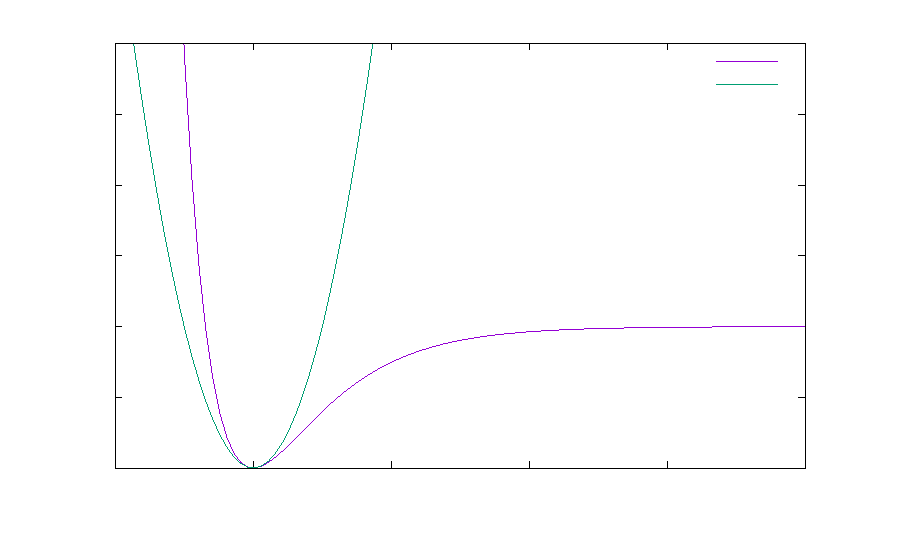
\includegraphics{THEX2b}}%
    \gplfronttext
  \end{picture}%
\endgroup

	\caption{}
	\label{fig:THEX2b}
\end{figure}
\missingfigure{Figuur van morse potential, taylor series en harmonic unit erop zetten}

\section{Exercise 3}
The characteristic frequency $ \omega $ of a harmonic spring with two masses is given by \cite{Taylor ofzo}
\begin{equation}
	\omega = \sqrt{\frac{k}{\mu}} 
\end{equation}
with $ k $ the spring constant and $ \mu = \left(\frac{1}{m_1} + \frac{1}{m_2}\right) $ the reduced mass. $ 1\unit{N/m} = 1.4393 \unit{kcal \, mol^{-1} \textrm{\AA}^{-2}} $


\todo{frequencies door rekenen en gebruiken omega = c*golfgetal}

\section{Exercise 4}
In a $ N $ dimensions the amount of periodic images is given by $ 3^N - 1 $. \todo{beetje uitleg geven}


\chapter{Molecular Dynamics of a Simple Liquid}
\todo[inline]{choose 1 of the master exercises}

\section{Exercise 1}
\todo[inline]{maken, mass: special == 1 -> mass = 1, special != 1 --> distribution 1}

\section{Exercise 2}
\subsection{a}
\todo[inline]{1.2 is voorbij cut-off, no repulsion when r>rmin}

\subsection{b}
\todo[inline]{maken}

\section{Exercise 3}
\subsection{a}
\todo[inline]{slides}

\subsection{b}
\todo[inline]{T = eps/kb, getallen invullen, slides, p = eps/sigma\^3}

\subsection{c}
\todo[inline]{sigma/characteristic time}

\section{Exercises 4}
\todo[inline]{sommatie van impulsen moet 0 zijn, Vcm = sum(mi vi)/sum(mi), vi = vi - Vcm, geimplementeerd in loop starting at r. 235.}

\section{Exercise 5}
\subsection{a}
\todo[inline]{Trivial}

\subsection{b}
\todo[inline]{N*(N-1)/2}

\section{Exercise 6}
\todo[inline]{r. 348 ff}

\section{Exercise 7}
\subsection{a}
\todo[inline]{position: use L MOD R such that 0<R<L}

\subsection{b}
\todo[inline]{26 (3\^N-1)}

\subsection{c}
\todo[inline]{interaction: use L MOD R such that -L/2<R<L/2 for each of the coordinates separately}

\section{Problem 1}
\begin{figure}
	\centering
	% GNUPLOT: LaTeX picture with Postscript
\begingroup
  \makeatletter
  \providecommand\color[2][]{%
    \GenericError{(gnuplot) \space\space\space\@spaces}{%
      Package color not loaded in conjunction with
      terminal option `colourtext'%
    }{See the gnuplot documentation for explanation.%
    }{Either use 'blacktext' in gnuplot or load the package
      color.sty in LaTeX.}%
    \renewcommand\color[2][]{}%
  }%
  \providecommand\includegraphics[2][]{%
    \GenericError{(gnuplot) \space\space\space\@spaces}{%
      Package graphicx or graphics not loaded%
    }{See the gnuplot documentation for explanation.%
    }{The gnuplot epslatex terminal needs graphicx.sty or graphics.sty.}%
    \renewcommand\includegraphics[2][]{}%
  }%
  \providecommand\rotatebox[2]{#2}%
  \@ifundefined{ifGPcolor}{%
    \newif\ifGPcolor
    \GPcolorfalse
  }{}%
  \@ifundefined{ifGPblacktext}{%
    \newif\ifGPblacktext
    \GPblacktexttrue
  }{}%
  % define a \g@addto@macro without @ in the name:
  \let\gplgaddtomacro\g@addto@macro
  % define empty templates for all commands taking text:
  \gdef\gplbacktext{}%
  \gdef\gplfronttext{}%
  \makeatother
  \ifGPblacktext
    % no textcolor at all
    \def\colorrgb#1{}%
    \def\colorgray#1{}%
  \else
    % gray or color?
    \ifGPcolor
      \def\colorrgb#1{\color[rgb]{#1}}%
      \def\colorgray#1{\color[gray]{#1}}%
      \expandafter\def\csname LTw\endcsname{\color{white}}%
      \expandafter\def\csname LTb\endcsname{\color{black}}%
      \expandafter\def\csname LTa\endcsname{\color{black}}%
      \expandafter\def\csname LT0\endcsname{\color[rgb]{1,0,0}}%
      \expandafter\def\csname LT1\endcsname{\color[rgb]{0,1,0}}%
      \expandafter\def\csname LT2\endcsname{\color[rgb]{0,0,1}}%
      \expandafter\def\csname LT3\endcsname{\color[rgb]{1,0,1}}%
      \expandafter\def\csname LT4\endcsname{\color[rgb]{0,1,1}}%
      \expandafter\def\csname LT5\endcsname{\color[rgb]{1,1,0}}%
      \expandafter\def\csname LT6\endcsname{\color[rgb]{0,0,0}}%
      \expandafter\def\csname LT7\endcsname{\color[rgb]{1,0.3,0}}%
      \expandafter\def\csname LT8\endcsname{\color[rgb]{0.5,0.5,0.5}}%
    \else
      % gray
      \def\colorrgb#1{\color{black}}%
      \def\colorgray#1{\color[gray]{#1}}%
      \expandafter\def\csname LTw\endcsname{\color{white}}%
      \expandafter\def\csname LTb\endcsname{\color{black}}%
      \expandafter\def\csname LTa\endcsname{\color{black}}%
      \expandafter\def\csname LT0\endcsname{\color{black}}%
      \expandafter\def\csname LT1\endcsname{\color{black}}%
      \expandafter\def\csname LT2\endcsname{\color{black}}%
      \expandafter\def\csname LT3\endcsname{\color{black}}%
      \expandafter\def\csname LT4\endcsname{\color{black}}%
      \expandafter\def\csname LT5\endcsname{\color{black}}%
      \expandafter\def\csname LT6\endcsname{\color{black}}%
      \expandafter\def\csname LT7\endcsname{\color{black}}%
      \expandafter\def\csname LT8\endcsname{\color{black}}%
    \fi
  \fi
    \setlength{\unitlength}{0.0500bp}%
    \ifx\gptboxheight\undefined%
      \newlength{\gptboxheight}%
      \newlength{\gptboxwidth}%
      \newsavebox{\gptboxtext}%
    \fi%
    \setlength{\fboxrule}{0.5pt}%
    \setlength{\fboxsep}{1pt}%
\begin{picture}(8496.00,3528.00)%
    \gplgaddtomacro\gplbacktext{%
      \csname LTb\endcsname%
      \put(733,907){\makebox(0,0){\strut{}$0$}}%
      \put(1376,826){\makebox(0,0){\strut{}$0.5$}}%
      \put(2020,745){\makebox(0,0){\strut{}$1$}}%
      \put(2870,759){\makebox(0,0){\strut{}$-0.5$}}%
      \put(3366,946){\makebox(0,0){\strut{}$0$}}%
      \put(3861,1132){\makebox(0,0){\strut{}$0.5$}}%
      \put(459,1306){\makebox(0,0)[r]{\strut{}$-0.1$}}%
      \put(459,1780){\makebox(0,0)[r]{\strut{}$0$}}%
      \put(459,2252){\makebox(0,0)[r]{\strut{}$0.1$}}%
      \put(-75,1780){\makebox(0,0){\strut{}z}}%
    }%
    \gplgaddtomacro\gplfronttext{%
      \csname LTb\endcsname%
      \put(1318,609){\makebox(0,0){\strut{}x}}%
      \put(3753,751){\makebox(0,0){\strut{}y}}%
      \put(-75,1780){\makebox(0,0){\strut{}z}}%
    }%
    \gplgaddtomacro\gplbacktext{%
      \csname LTb\endcsname%
      \put(4540,664){\makebox(0,0)[r]{\strut{}$-1$}}%
      \put(4540,947){\makebox(0,0)[r]{\strut{}$-0.8$}}%
      \put(4540,1229){\makebox(0,0)[r]{\strut{}$-0.6$}}%
      \put(4540,1512){\makebox(0,0)[r]{\strut{}$-0.4$}}%
      \put(4540,1795){\makebox(0,0)[r]{\strut{}$-0.2$}}%
      \put(4540,2078){\makebox(0,0)[r]{\strut{}$0$}}%
      \put(4540,2361){\makebox(0,0)[r]{\strut{}$0.2$}}%
      \put(4540,2643){\makebox(0,0)[r]{\strut{}$0.4$}}%
      \put(4540,2926){\makebox(0,0)[r]{\strut{}$0.6$}}%
      \put(4540,3209){\makebox(0,0)[r]{\strut{}$0.8$}}%
      \put(4672,373){\makebox(0,0){\strut{}$0$}}%
      \put(5420,373){\makebox(0,0){\strut{}$2$}}%
      \put(6167,373){\makebox(0,0){\strut{}$4$}}%
      \put(6915,373){\makebox(0,0){\strut{}$6$}}%
      \put(7662,373){\makebox(0,0){\strut{}$8$}}%
      \put(8410,373){\makebox(0,0){\strut{}$10$}}%
    }%
    \gplgaddtomacro\gplfronttext{%
      \csname LTb\endcsname%
      \put(3968,1901){\rotatebox{-270}{\makebox(0,0){\strut{}energy}}}%
      \put(6541,208){\makebox(0,0){\strut{}time t}}%
      \csname LTb\endcsname%
      \put(7480,2745){\makebox(0,0)[r]{\strut{}Kinetic energy}}%
      \csname LTb\endcsname%
      \put(7480,2525){\makebox(0,0)[r]{\strut{}Potential energy}}%
      \csname LTb\endcsname%
      \put(7480,2305){\makebox(0,0)[r]{\strut{}Total energy}}%
    }%
    \gplbacktext
    \put(0,0){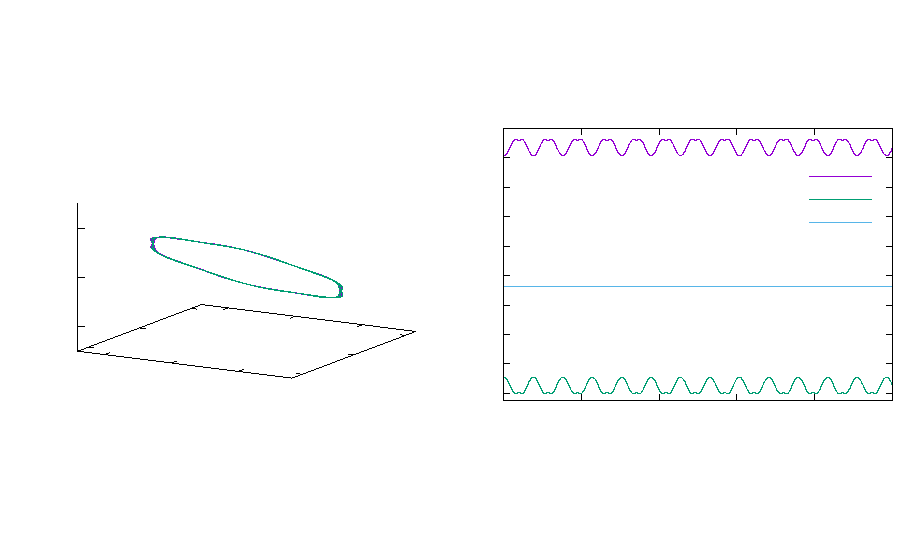
\includegraphics{MDSLP1}}%
    \gplfronttext
  \end{picture}%
\endgroup

	\caption{}
	\label{fig:MDSLP1}
\end{figure}

\section{Problem 2}
\begin{figure}
	\centering
	% GNUPLOT: LaTeX picture with Postscript
\begingroup
  \makeatletter
  \providecommand\color[2][]{%
    \GenericError{(gnuplot) \space\space\space\@spaces}{%
      Package color not loaded in conjunction with
      terminal option `colourtext'%
    }{See the gnuplot documentation for explanation.%
    }{Either use 'blacktext' in gnuplot or load the package
      color.sty in LaTeX.}%
    \renewcommand\color[2][]{}%
  }%
  \providecommand\includegraphics[2][]{%
    \GenericError{(gnuplot) \space\space\space\@spaces}{%
      Package graphicx or graphics not loaded%
    }{See the gnuplot documentation for explanation.%
    }{The gnuplot epslatex terminal needs graphicx.sty or graphics.sty.}%
    \renewcommand\includegraphics[2][]{}%
  }%
  \providecommand\rotatebox[2]{#2}%
  \@ifundefined{ifGPcolor}{%
    \newif\ifGPcolor
    \GPcolorfalse
  }{}%
  \@ifundefined{ifGPblacktext}{%
    \newif\ifGPblacktext
    \GPblacktexttrue
  }{}%
  % define a \g@addto@macro without @ in the name:
  \let\gplgaddtomacro\g@addto@macro
  % define empty templates for all commands taking text:
  \gdef\gplbacktext{}%
  \gdef\gplfronttext{}%
  \makeatother
  \ifGPblacktext
    % no textcolor at all
    \def\colorrgb#1{}%
    \def\colorgray#1{}%
  \else
    % gray or color?
    \ifGPcolor
      \def\colorrgb#1{\color[rgb]{#1}}%
      \def\colorgray#1{\color[gray]{#1}}%
      \expandafter\def\csname LTw\endcsname{\color{white}}%
      \expandafter\def\csname LTb\endcsname{\color{black}}%
      \expandafter\def\csname LTa\endcsname{\color{black}}%
      \expandafter\def\csname LT0\endcsname{\color[rgb]{1,0,0}}%
      \expandafter\def\csname LT1\endcsname{\color[rgb]{0,1,0}}%
      \expandafter\def\csname LT2\endcsname{\color[rgb]{0,0,1}}%
      \expandafter\def\csname LT3\endcsname{\color[rgb]{1,0,1}}%
      \expandafter\def\csname LT4\endcsname{\color[rgb]{0,1,1}}%
      \expandafter\def\csname LT5\endcsname{\color[rgb]{1,1,0}}%
      \expandafter\def\csname LT6\endcsname{\color[rgb]{0,0,0}}%
      \expandafter\def\csname LT7\endcsname{\color[rgb]{1,0.3,0}}%
      \expandafter\def\csname LT8\endcsname{\color[rgb]{0.5,0.5,0.5}}%
    \else
      % gray
      \def\colorrgb#1{\color{black}}%
      \def\colorgray#1{\color[gray]{#1}}%
      \expandafter\def\csname LTw\endcsname{\color{white}}%
      \expandafter\def\csname LTb\endcsname{\color{black}}%
      \expandafter\def\csname LTa\endcsname{\color{black}}%
      \expandafter\def\csname LT0\endcsname{\color{black}}%
      \expandafter\def\csname LT1\endcsname{\color{black}}%
      \expandafter\def\csname LT2\endcsname{\color{black}}%
      \expandafter\def\csname LT3\endcsname{\color{black}}%
      \expandafter\def\csname LT4\endcsname{\color{black}}%
      \expandafter\def\csname LT5\endcsname{\color{black}}%
      \expandafter\def\csname LT6\endcsname{\color{black}}%
      \expandafter\def\csname LT7\endcsname{\color{black}}%
      \expandafter\def\csname LT8\endcsname{\color{black}}%
    \fi
  \fi
    \setlength{\unitlength}{0.0500bp}%
    \ifx\gptboxheight\undefined%
      \newlength{\gptboxheight}%
      \newlength{\gptboxwidth}%
      \newsavebox{\gptboxtext}%
    \fi%
    \setlength{\fboxrule}{0.5pt}%
    \setlength{\fboxsep}{1pt}%
\begin{picture}(8496.00,3528.00)%
    \gplgaddtomacro\gplbacktext{%
      \csname LTb\endcsname%
      \put(663,916){\makebox(0,0){\strut{}$-0.5$}}%
      \put(1131,857){\makebox(0,0){\strut{}$0$}}%
      \put(1599,798){\makebox(0,0){\strut{}$0.5$}}%
      \put(2067,739){\makebox(0,0){\strut{}$1$}}%
      \put(2534,681){\makebox(0,0){\strut{}$1.5$}}%
      \put(2879,763){\makebox(0,0){\strut{}$-0.5$}}%
      \put(3149,864){\makebox(0,0){\strut{}$0$}}%
      \put(3420,966){\makebox(0,0){\strut{}$0.5$}}%
      \put(3690,1068){\makebox(0,0){\strut{}$1$}}%
      \put(3960,1170){\makebox(0,0){\strut{}$1.5$}}%
      \put(459,1069){\makebox(0,0)[r]{\strut{}$-0.6$}}%
      \put(459,1272){\makebox(0,0)[r]{\strut{}$-0.4$}}%
      \put(459,1475){\makebox(0,0)[r]{\strut{}$-0.2$}}%
      \put(459,1678){\makebox(0,0)[r]{\strut{}$0$}}%
      \put(459,1880){\makebox(0,0)[r]{\strut{}$0.2$}}%
      \put(459,2083){\makebox(0,0)[r]{\strut{}$0.4$}}%
      \put(459,2286){\makebox(0,0)[r]{\strut{}$0.6$}}%
      \put(459,2489){\makebox(0,0)[r]{\strut{}$0.8$}}%
      \put(-75,1780){\makebox(0,0){\strut{}z}}%
    }%
    \gplgaddtomacro\gplfronttext{%
      \csname LTb\endcsname%
      \put(1318,609){\makebox(0,0){\strut{}x}}%
      \put(3753,751){\makebox(0,0){\strut{}y}}%
      \put(-75,1780){\makebox(0,0){\strut{}z}}%
    }%
    \gplgaddtomacro\gplbacktext{%
      \csname LTb\endcsname%
      \put(4540,593){\makebox(0,0)[r]{\strut{}$-3$}}%
      \put(4540,855){\makebox(0,0)[r]{\strut{}$-2.5$}}%
      \put(4540,1116){\makebox(0,0)[r]{\strut{}$-2$}}%
      \put(4540,1378){\makebox(0,0)[r]{\strut{}$-1.5$}}%
      \put(4540,1639){\makebox(0,0)[r]{\strut{}$-1$}}%
      \put(4540,1901){\makebox(0,0)[r]{\strut{}$-0.5$}}%
      \put(4540,2163){\makebox(0,0)[r]{\strut{}$0$}}%
      \put(4540,2424){\makebox(0,0)[r]{\strut{}$0.5$}}%
      \put(4540,2686){\makebox(0,0)[r]{\strut{}$1$}}%
      \put(4540,2947){\makebox(0,0)[r]{\strut{}$1.5$}}%
      \put(4540,3209){\makebox(0,0)[r]{\strut{}$2$}}%
      \put(4672,373){\makebox(0,0){\strut{}$0$}}%
      \put(5420,373){\makebox(0,0){\strut{}$2$}}%
      \put(6167,373){\makebox(0,0){\strut{}$4$}}%
      \put(6915,373){\makebox(0,0){\strut{}$6$}}%
      \put(7662,373){\makebox(0,0){\strut{}$8$}}%
      \put(8410,373){\makebox(0,0){\strut{}$10$}}%
    }%
    \gplgaddtomacro\gplfronttext{%
      \csname LTb\endcsname%
      \put(3968,1901){\rotatebox{-270}{\makebox(0,0){\strut{}energy}}}%
      \put(6541,208){\makebox(0,0){\strut{}time t}}%
      \csname LTb\endcsname%
      \put(7480,2210){\makebox(0,0)[r]{\strut{}Kinetic energy}}%
      \csname LTb\endcsname%
      \put(7480,1990){\makebox(0,0)[r]{\strut{}Potential energy}}%
      \csname LTb\endcsname%
      \put(7480,1770){\makebox(0,0)[r]{\strut{}Total energy}}%
    }%
    \gplbacktext
    \put(0,0){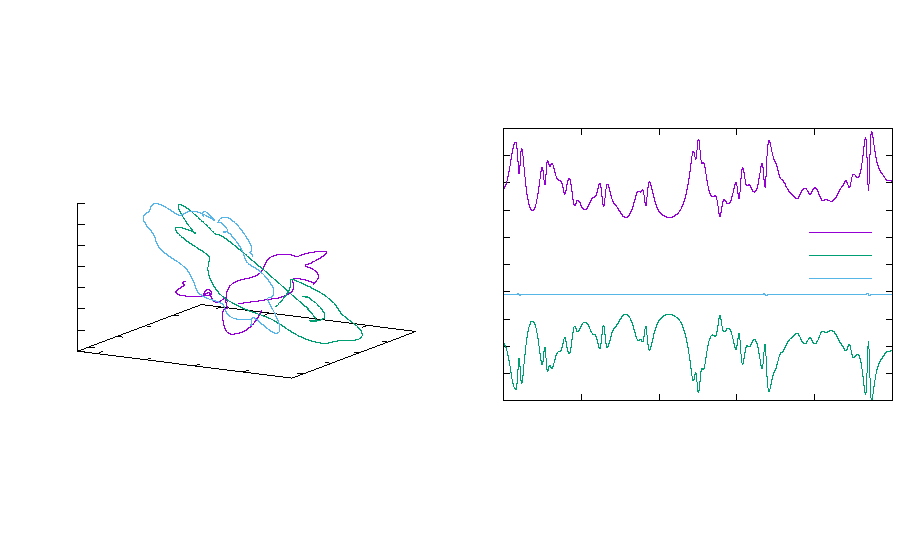
\includegraphics{MDSLP2}}%
    \gplfronttext
  \end{picture}%
\endgroup

	\caption{}
	\label{fig:MDSLP2}
\end{figure}

\section{Problem 3}
\begin{figure}
	\centering
	% GNUPLOT: LaTeX picture with Postscript
\begingroup
  \makeatletter
  \providecommand\color[2][]{%
    \GenericError{(gnuplot) \space\space\space\@spaces}{%
      Package color not loaded in conjunction with
      terminal option `colourtext'%
    }{See the gnuplot documentation for explanation.%
    }{Either use 'blacktext' in gnuplot or load the package
      color.sty in LaTeX.}%
    \renewcommand\color[2][]{}%
  }%
  \providecommand\includegraphics[2][]{%
    \GenericError{(gnuplot) \space\space\space\@spaces}{%
      Package graphicx or graphics not loaded%
    }{See the gnuplot documentation for explanation.%
    }{The gnuplot epslatex terminal needs graphicx.sty or graphics.sty.}%
    \renewcommand\includegraphics[2][]{}%
  }%
  \providecommand\rotatebox[2]{#2}%
  \@ifundefined{ifGPcolor}{%
    \newif\ifGPcolor
    \GPcolorfalse
  }{}%
  \@ifundefined{ifGPblacktext}{%
    \newif\ifGPblacktext
    \GPblacktexttrue
  }{}%
  % define a \g@addto@macro without @ in the name:
  \let\gplgaddtomacro\g@addto@macro
  % define empty templates for all commands taking text:
  \gdef\gplbacktext{}%
  \gdef\gplfronttext{}%
  \makeatother
  \ifGPblacktext
    % no textcolor at all
    \def\colorrgb#1{}%
    \def\colorgray#1{}%
  \else
    % gray or color?
    \ifGPcolor
      \def\colorrgb#1{\color[rgb]{#1}}%
      \def\colorgray#1{\color[gray]{#1}}%
      \expandafter\def\csname LTw\endcsname{\color{white}}%
      \expandafter\def\csname LTb\endcsname{\color{black}}%
      \expandafter\def\csname LTa\endcsname{\color{black}}%
      \expandafter\def\csname LT0\endcsname{\color[rgb]{1,0,0}}%
      \expandafter\def\csname LT1\endcsname{\color[rgb]{0,1,0}}%
      \expandafter\def\csname LT2\endcsname{\color[rgb]{0,0,1}}%
      \expandafter\def\csname LT3\endcsname{\color[rgb]{1,0,1}}%
      \expandafter\def\csname LT4\endcsname{\color[rgb]{0,1,1}}%
      \expandafter\def\csname LT5\endcsname{\color[rgb]{1,1,0}}%
      \expandafter\def\csname LT6\endcsname{\color[rgb]{0,0,0}}%
      \expandafter\def\csname LT7\endcsname{\color[rgb]{1,0.3,0}}%
      \expandafter\def\csname LT8\endcsname{\color[rgb]{0.5,0.5,0.5}}%
    \else
      % gray
      \def\colorrgb#1{\color{black}}%
      \def\colorgray#1{\color[gray]{#1}}%
      \expandafter\def\csname LTw\endcsname{\color{white}}%
      \expandafter\def\csname LTb\endcsname{\color{black}}%
      \expandafter\def\csname LTa\endcsname{\color{black}}%
      \expandafter\def\csname LT0\endcsname{\color{black}}%
      \expandafter\def\csname LT1\endcsname{\color{black}}%
      \expandafter\def\csname LT2\endcsname{\color{black}}%
      \expandafter\def\csname LT3\endcsname{\color{black}}%
      \expandafter\def\csname LT4\endcsname{\color{black}}%
      \expandafter\def\csname LT5\endcsname{\color{black}}%
      \expandafter\def\csname LT6\endcsname{\color{black}}%
      \expandafter\def\csname LT7\endcsname{\color{black}}%
      \expandafter\def\csname LT8\endcsname{\color{black}}%
    \fi
  \fi
    \setlength{\unitlength}{0.0500bp}%
    \ifx\gptboxheight\undefined%
      \newlength{\gptboxheight}%
      \newlength{\gptboxwidth}%
      \newsavebox{\gptboxtext}%
    \fi%
    \setlength{\fboxrule}{0.5pt}%
    \setlength{\fboxsep}{1pt}%
\begin{picture}(8496.00,5040.00)%
    \gplgaddtomacro\gplbacktext{%
      \csname LTb\endcsname%
      \put(475,1695){\makebox(0,0){\strut{}$-2$}}%
      \put(770,1658){\makebox(0,0){\strut{}$-1$}}%
      \put(1064,1621){\makebox(0,0){\strut{}$0$}}%
      \put(1358,1584){\makebox(0,0){\strut{}$1$}}%
      \put(1652,1548){\makebox(0,0){\strut{}$2$}}%
      \put(1947,1511){\makebox(0,0){\strut{}$3$}}%
      \put(2240,1474){\makebox(0,0){\strut{}$4$}}%
      \put(2534,1437){\makebox(0,0){\strut{}$5$}}%
      \put(2771,1478){\makebox(0,0){\strut{}$-1$}}%
      \put(3068,1590){\makebox(0,0){\strut{}$0$}}%
      \put(3366,1702){\makebox(0,0){\strut{}$1$}}%
      \put(3663,1814){\makebox(0,0){\strut{}$2$}}%
      \put(3960,1926){\makebox(0,0){\strut{}$3$}}%
      \put(459,1983){\makebox(0,0)[r]{\strut{}$-2$}}%
      \put(459,2299){\makebox(0,0)[r]{\strut{}$-1$}}%
      \put(459,2615){\makebox(0,0)[r]{\strut{}$0$}}%
      \put(459,2930){\makebox(0,0)[r]{\strut{}$1$}}%
      \put(459,3245){\makebox(0,0)[r]{\strut{}$2$}}%
      \put(-75,2536){\makebox(0,0){\strut{}z}}%
    }%
    \gplgaddtomacro\gplfronttext{%
      \csname LTb\endcsname%
      \put(1318,1365){\makebox(0,0){\strut{}x}}%
      \put(3753,1507){\makebox(0,0){\strut{}y}}%
      \put(-75,2536){\makebox(0,0){\strut{}z}}%
    }%
    \gplgaddtomacro\gplbacktext{%
      \csname LTb\endcsname%
      \put(4540,1587){\makebox(0,0)[r]{\strut{}$-4$}}%
      \put(4540,1927){\makebox(0,0)[r]{\strut{}$-3$}}%
      \put(4540,2266){\makebox(0,0)[r]{\strut{}$-2$}}%
      \put(4540,2606){\makebox(0,0)[r]{\strut{}$-1$}}%
      \put(4540,2946){\makebox(0,0)[r]{\strut{}$0$}}%
      \put(4540,3286){\makebox(0,0)[r]{\strut{}$1$}}%
      \put(4540,3625){\makebox(0,0)[r]{\strut{}$2$}}%
      \put(4540,3965){\makebox(0,0)[r]{\strut{}$3$}}%
      \put(4672,1129){\makebox(0,0){\strut{}$0$}}%
      \put(5420,1129){\makebox(0,0){\strut{}$2$}}%
      \put(6167,1129){\makebox(0,0){\strut{}$4$}}%
      \put(6915,1129){\makebox(0,0){\strut{}$6$}}%
      \put(7662,1129){\makebox(0,0){\strut{}$8$}}%
      \put(8410,1129){\makebox(0,0){\strut{}$10$}}%
    }%
    \gplgaddtomacro\gplfronttext{%
      \csname LTb\endcsname%
      \put(4232,2657){\rotatebox{-270}{\makebox(0,0){\strut{}energy}}}%
      \put(6541,964){\makebox(0,0){\strut{}time t}}%
      \csname LTb\endcsname%
      \put(7480,3023){\makebox(0,0)[r]{\strut{}Kinetic energy}}%
      \csname LTb\endcsname%
      \put(7480,2803){\makebox(0,0)[r]{\strut{}Potential energy}}%
      \csname LTb\endcsname%
      \put(7480,2583){\makebox(0,0)[r]{\strut{}Total energy}}%
    }%
    \gplbacktext
    \put(0,0){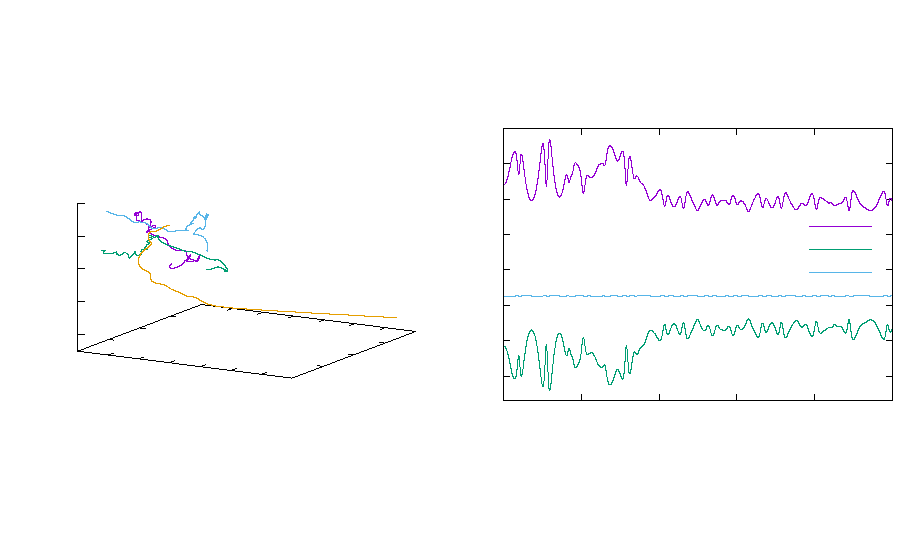
\includegraphics{MDSLP3N4}}%
    \gplfronttext
  \end{picture}%
\endgroup

	\caption{}
	\label{fig:MDSLP3N4}
\end{figure}

\begin{figure}
	\centering
	% GNUPLOT: LaTeX picture with Postscript
\begingroup
  \makeatletter
  \providecommand\color[2][]{%
    \GenericError{(gnuplot) \space\space\space\@spaces}{%
      Package color not loaded in conjunction with
      terminal option `colourtext'%
    }{See the gnuplot documentation for explanation.%
    }{Either use 'blacktext' in gnuplot or load the package
      color.sty in LaTeX.}%
    \renewcommand\color[2][]{}%
  }%
  \providecommand\includegraphics[2][]{%
    \GenericError{(gnuplot) \space\space\space\@spaces}{%
      Package graphicx or graphics not loaded%
    }{See the gnuplot documentation for explanation.%
    }{The gnuplot epslatex terminal needs graphicx.sty or graphics.sty.}%
    \renewcommand\includegraphics[2][]{}%
  }%
  \providecommand\rotatebox[2]{#2}%
  \@ifundefined{ifGPcolor}{%
    \newif\ifGPcolor
    \GPcolorfalse
  }{}%
  \@ifundefined{ifGPblacktext}{%
    \newif\ifGPblacktext
    \GPblacktexttrue
  }{}%
  % define a \g@addto@macro without @ in the name:
  \let\gplgaddtomacro\g@addto@macro
  % define empty templates for all commands taking text:
  \gdef\gplbacktext{}%
  \gdef\gplfronttext{}%
  \makeatother
  \ifGPblacktext
    % no textcolor at all
    \def\colorrgb#1{}%
    \def\colorgray#1{}%
  \else
    % gray or color?
    \ifGPcolor
      \def\colorrgb#1{\color[rgb]{#1}}%
      \def\colorgray#1{\color[gray]{#1}}%
      \expandafter\def\csname LTw\endcsname{\color{white}}%
      \expandafter\def\csname LTb\endcsname{\color{black}}%
      \expandafter\def\csname LTa\endcsname{\color{black}}%
      \expandafter\def\csname LT0\endcsname{\color[rgb]{1,0,0}}%
      \expandafter\def\csname LT1\endcsname{\color[rgb]{0,1,0}}%
      \expandafter\def\csname LT2\endcsname{\color[rgb]{0,0,1}}%
      \expandafter\def\csname LT3\endcsname{\color[rgb]{1,0,1}}%
      \expandafter\def\csname LT4\endcsname{\color[rgb]{0,1,1}}%
      \expandafter\def\csname LT5\endcsname{\color[rgb]{1,1,0}}%
      \expandafter\def\csname LT6\endcsname{\color[rgb]{0,0,0}}%
      \expandafter\def\csname LT7\endcsname{\color[rgb]{1,0.3,0}}%
      \expandafter\def\csname LT8\endcsname{\color[rgb]{0.5,0.5,0.5}}%
    \else
      % gray
      \def\colorrgb#1{\color{black}}%
      \def\colorgray#1{\color[gray]{#1}}%
      \expandafter\def\csname LTw\endcsname{\color{white}}%
      \expandafter\def\csname LTb\endcsname{\color{black}}%
      \expandafter\def\csname LTa\endcsname{\color{black}}%
      \expandafter\def\csname LT0\endcsname{\color{black}}%
      \expandafter\def\csname LT1\endcsname{\color{black}}%
      \expandafter\def\csname LT2\endcsname{\color{black}}%
      \expandafter\def\csname LT3\endcsname{\color{black}}%
      \expandafter\def\csname LT4\endcsname{\color{black}}%
      \expandafter\def\csname LT5\endcsname{\color{black}}%
      \expandafter\def\csname LT6\endcsname{\color{black}}%
      \expandafter\def\csname LT7\endcsname{\color{black}}%
      \expandafter\def\csname LT8\endcsname{\color{black}}%
    \fi
  \fi
    \setlength{\unitlength}{0.0500bp}%
    \ifx\gptboxheight\undefined%
      \newlength{\gptboxheight}%
      \newlength{\gptboxwidth}%
      \newsavebox{\gptboxtext}%
    \fi%
    \setlength{\fboxrule}{0.5pt}%
    \setlength{\fboxsep}{1pt}%
\begin{picture}(8496.00,5040.00)%
    \gplgaddtomacro\gplbacktext{%
      \csname LTb\endcsname%
      \put(770,1658){\makebox(0,0){\strut{}$-1$}}%
      \put(1358,1584){\makebox(0,0){\strut{}$0$}}%
      \put(1947,1511){\makebox(0,0){\strut{}$1$}}%
      \put(2534,1437){\makebox(0,0){\strut{}$2$}}%
      \put(2771,1478){\makebox(0,0){\strut{}$-1$}}%
      \put(3167,1627){\makebox(0,0){\strut{}$0$}}%
      \put(3564,1777){\makebox(0,0){\strut{}$1$}}%
      \put(3960,1926){\makebox(0,0){\strut{}$2$}}%
      \put(459,1825){\makebox(0,0)[r]{\strut{}$-1$}}%
      \put(459,2231){\makebox(0,0)[r]{\strut{}$0$}}%
      \put(459,2636){\makebox(0,0)[r]{\strut{}$1$}}%
      \put(459,3042){\makebox(0,0)[r]{\strut{}$2$}}%
      \put(-75,2536){\makebox(0,0){\strut{}z}}%
    }%
    \gplgaddtomacro\gplfronttext{%
      \csname LTb\endcsname%
      \put(1318,1365){\makebox(0,0){\strut{}x}}%
      \put(3753,1507){\makebox(0,0){\strut{}y}}%
      \put(-75,2536){\makebox(0,0){\strut{}z}}%
    }%
    \gplgaddtomacro\gplbacktext{%
      \csname LTb\endcsname%
      \put(4540,1587){\makebox(0,0)[r]{\strut{}$-6$}}%
      \put(4540,2062){\makebox(0,0)[r]{\strut{}$-4$}}%
      \put(4540,2538){\makebox(0,0)[r]{\strut{}$-2$}}%
      \put(4540,3014){\makebox(0,0)[r]{\strut{}$0$}}%
      \put(4540,3489){\makebox(0,0)[r]{\strut{}$2$}}%
      \put(4540,3965){\makebox(0,0)[r]{\strut{}$4$}}%
      \put(4672,1129){\makebox(0,0){\strut{}$0$}}%
      \put(5420,1129){\makebox(0,0){\strut{}$2$}}%
      \put(6167,1129){\makebox(0,0){\strut{}$4$}}%
      \put(6915,1129){\makebox(0,0){\strut{}$6$}}%
      \put(7662,1129){\makebox(0,0){\strut{}$8$}}%
      \put(8410,1129){\makebox(0,0){\strut{}$10$}}%
    }%
    \gplgaddtomacro\gplfronttext{%
      \csname LTb\endcsname%
      \put(4232,2657){\rotatebox{-270}{\makebox(0,0){\strut{}energy}}}%
      \put(6541,964){\makebox(0,0){\strut{}time t}}%
      \csname LTb\endcsname%
      \put(7480,3035){\makebox(0,0)[r]{\strut{}Kinetic energy}}%
      \csname LTb\endcsname%
      \put(7480,2815){\makebox(0,0)[r]{\strut{}Potential energy}}%
      \csname LTb\endcsname%
      \put(7480,2595){\makebox(0,0)[r]{\strut{}Total energy}}%
    }%
    \gplbacktext
    \put(0,0){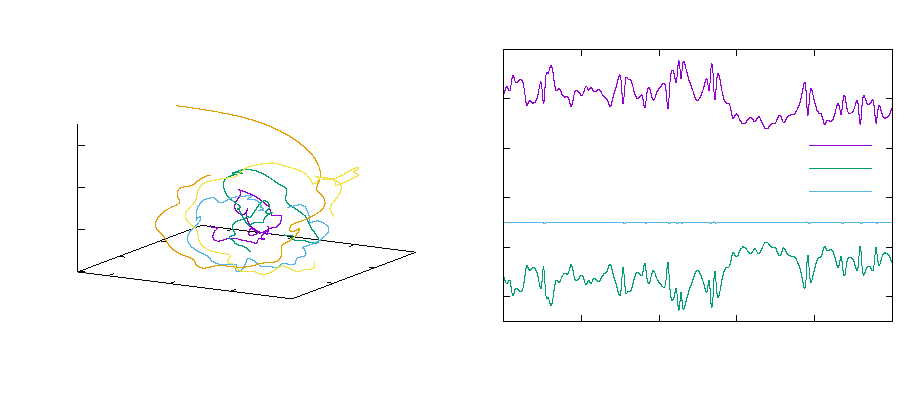
\includegraphics{MDSLP3N5}}%
    \gplfronttext
  \end{picture}%
\endgroup

	\caption{}
	\label{fig:MDSLP3N5}
\end{figure}

\begin{figure}
	\centering
	% GNUPLOT: LaTeX picture with Postscript
\begingroup
  \makeatletter
  \providecommand\color[2][]{%
    \GenericError{(gnuplot) \space\space\space\@spaces}{%
      Package color not loaded in conjunction with
      terminal option `colourtext'%
    }{See the gnuplot documentation for explanation.%
    }{Either use 'blacktext' in gnuplot or load the package
      color.sty in LaTeX.}%
    \renewcommand\color[2][]{}%
  }%
  \providecommand\includegraphics[2][]{%
    \GenericError{(gnuplot) \space\space\space\@spaces}{%
      Package graphicx or graphics not loaded%
    }{See the gnuplot documentation for explanation.%
    }{The gnuplot epslatex terminal needs graphicx.sty or graphics.sty.}%
    \renewcommand\includegraphics[2][]{}%
  }%
  \providecommand\rotatebox[2]{#2}%
  \@ifundefined{ifGPcolor}{%
    \newif\ifGPcolor
    \GPcolorfalse
  }{}%
  \@ifundefined{ifGPblacktext}{%
    \newif\ifGPblacktext
    \GPblacktexttrue
  }{}%
  % define a \g@addto@macro without @ in the name:
  \let\gplgaddtomacro\g@addto@macro
  % define empty templates for all commands taking text:
  \gdef\gplbacktext{}%
  \gdef\gplfronttext{}%
  \makeatother
  \ifGPblacktext
    % no textcolor at all
    \def\colorrgb#1{}%
    \def\colorgray#1{}%
  \else
    % gray or color?
    \ifGPcolor
      \def\colorrgb#1{\color[rgb]{#1}}%
      \def\colorgray#1{\color[gray]{#1}}%
      \expandafter\def\csname LTw\endcsname{\color{white}}%
      \expandafter\def\csname LTb\endcsname{\color{black}}%
      \expandafter\def\csname LTa\endcsname{\color{black}}%
      \expandafter\def\csname LT0\endcsname{\color[rgb]{1,0,0}}%
      \expandafter\def\csname LT1\endcsname{\color[rgb]{0,1,0}}%
      \expandafter\def\csname LT2\endcsname{\color[rgb]{0,0,1}}%
      \expandafter\def\csname LT3\endcsname{\color[rgb]{1,0,1}}%
      \expandafter\def\csname LT4\endcsname{\color[rgb]{0,1,1}}%
      \expandafter\def\csname LT5\endcsname{\color[rgb]{1,1,0}}%
      \expandafter\def\csname LT6\endcsname{\color[rgb]{0,0,0}}%
      \expandafter\def\csname LT7\endcsname{\color[rgb]{1,0.3,0}}%
      \expandafter\def\csname LT8\endcsname{\color[rgb]{0.5,0.5,0.5}}%
    \else
      % gray
      \def\colorrgb#1{\color{black}}%
      \def\colorgray#1{\color[gray]{#1}}%
      \expandafter\def\csname LTw\endcsname{\color{white}}%
      \expandafter\def\csname LTb\endcsname{\color{black}}%
      \expandafter\def\csname LTa\endcsname{\color{black}}%
      \expandafter\def\csname LT0\endcsname{\color{black}}%
      \expandafter\def\csname LT1\endcsname{\color{black}}%
      \expandafter\def\csname LT2\endcsname{\color{black}}%
      \expandafter\def\csname LT3\endcsname{\color{black}}%
      \expandafter\def\csname LT4\endcsname{\color{black}}%
      \expandafter\def\csname LT5\endcsname{\color{black}}%
      \expandafter\def\csname LT6\endcsname{\color{black}}%
      \expandafter\def\csname LT7\endcsname{\color{black}}%
      \expandafter\def\csname LT8\endcsname{\color{black}}%
    \fi
  \fi
    \setlength{\unitlength}{0.0500bp}%
    \ifx\gptboxheight\undefined%
      \newlength{\gptboxheight}%
      \newlength{\gptboxwidth}%
      \newsavebox{\gptboxtext}%
    \fi%
    \setlength{\fboxrule}{0.5pt}%
    \setlength{\fboxsep}{1pt}%
\begin{picture}(8496.00,3528.00)%
    \gplgaddtomacro\gplbacktext{%
      \csname LTb\endcsname%
      \put(819,896){\makebox(0,0){\strut{}$0$}}%
      \put(1505,810){\makebox(0,0){\strut{}$1$}}%
      \put(2192,724){\makebox(0,0){\strut{}$2$}}%
      \put(2771,722){\makebox(0,0){\strut{}$-1$}}%
      \put(3167,871){\makebox(0,0){\strut{}$0$}}%
      \put(3564,1021){\makebox(0,0){\strut{}$1$}}%
      \put(3960,1170){\makebox(0,0){\strut{}$2$}}%
      \put(459,1069){\makebox(0,0)[r]{\strut{}$-1$}}%
      \put(459,1475){\makebox(0,0)[r]{\strut{}$0$}}%
      \put(459,1880){\makebox(0,0)[r]{\strut{}$1$}}%
      \put(459,2286){\makebox(0,0)[r]{\strut{}$2$}}%
      \put(-75,1780){\makebox(0,0){\strut{}z}}%
    }%
    \gplgaddtomacro\gplfronttext{%
      \csname LTb\endcsname%
      \put(1318,609){\makebox(0,0){\strut{}x}}%
      \put(3753,751){\makebox(0,0){\strut{}y}}%
      \put(-75,1780){\makebox(0,0){\strut{}z}}%
    }%
    \gplgaddtomacro\gplbacktext{%
      \csname LTb\endcsname%
      \put(4540,747){\makebox(0,0)[r]{\strut{}$-10$}}%
      \put(4540,1055){\makebox(0,0)[r]{\strut{}$-8$}}%
      \put(4540,1362){\makebox(0,0)[r]{\strut{}$-6$}}%
      \put(4540,1670){\makebox(0,0)[r]{\strut{}$-4$}}%
      \put(4540,1978){\makebox(0,0)[r]{\strut{}$-2$}}%
      \put(4540,2286){\makebox(0,0)[r]{\strut{}$0$}}%
      \put(4540,2593){\makebox(0,0)[r]{\strut{}$2$}}%
      \put(4540,2901){\makebox(0,0)[r]{\strut{}$4$}}%
      \put(4540,3209){\makebox(0,0)[r]{\strut{}$6$}}%
      \put(4672,373){\makebox(0,0){\strut{}$0$}}%
      \put(5420,373){\makebox(0,0){\strut{}$2$}}%
      \put(6167,373){\makebox(0,0){\strut{}$4$}}%
      \put(6915,373){\makebox(0,0){\strut{}$6$}}%
      \put(7662,373){\makebox(0,0){\strut{}$8$}}%
      \put(8410,373){\makebox(0,0){\strut{}$10$}}%
    }%
    \gplgaddtomacro\gplfronttext{%
      \csname LTb\endcsname%
      \put(4100,1901){\rotatebox{-270}{\makebox(0,0){\strut{}energy}}}%
      \put(6541,208){\makebox(0,0){\strut{}time t}}%
      \csname LTb\endcsname%
      \put(7480,2260){\makebox(0,0)[r]{\strut{}Kinetic energy}}%
      \csname LTb\endcsname%
      \put(7480,2040){\makebox(0,0)[r]{\strut{}Potential energy}}%
      \csname LTb\endcsname%
      \put(7480,1820){\makebox(0,0)[r]{\strut{}Total energy}}%
    }%
    \gplbacktext
    \put(0,0){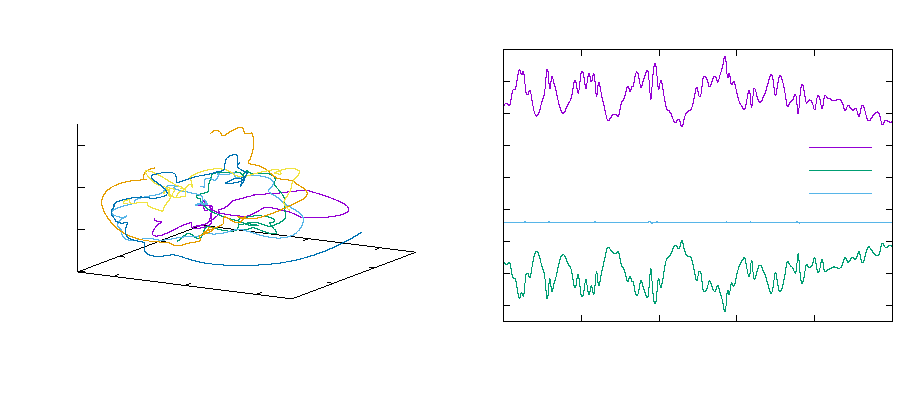
\includegraphics{MDSLP3N6}}%
    \gplfronttext
  \end{picture}%
\endgroup

	\caption{}
	\label{fig:MDSLP3N6}
\end{figure}

\insertbibliography
%\begin{appendices}
%% appendices hier
%
%
%\end{appendices}


\end{document}